\documentclass[tikz,border=6pt]{standalone}
\usepackage{tikz}
\usetikzlibrary{arrows.meta}
\definecolor{nebula}{HTML}{6366F1}
\definecolor{spark}{HTML}{14B8A6}
\definecolor{ink}{HTML}{334155}
\begin{document}
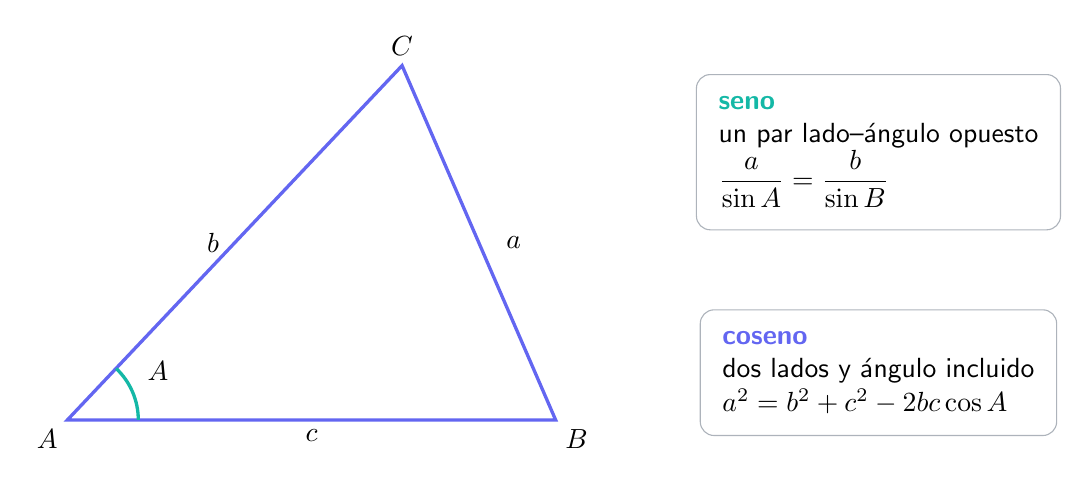
\begin{tikzpicture}[font=\sffamily,>=Latex]
  \coordinate (A) at (0,0); \coordinate (B) at (6.2,0); \coordinate (C) at (4.25,4.5);
  \draw[very thick,nebula] (A)--(B)--(C)--cycle;
  \node[below] at (3.1,0) {$c$};
  \node[right] at (5.45,2.25) {$a$};
  \node[left] at (2.05,2.25) {$b$};
  \node[below left] at (A) {$A$}; \node[below right] at (B) {$B$}; \node[above] at (C) {$C$};
  \draw[spark,very thick] (0.9,0) arc[start angle=0,end angle=46.6,radius=0.9];
  \node[fill=white] at (1.15,0.62) {$A$};
  \node[align=left,draw=ink!40,rounded corners=5pt,inner sep=8pt] at (10.3,3.4) {\textcolor{spark}{\bfseries seno}\\un par lado--\'angulo opuesto\\$\displaystyle \frac a{\sin A}=\frac b{\sin B}$};
  \node[align=left,draw=ink!40,rounded corners=5pt,inner sep=8pt] at (10.3,0.6) {\textcolor{nebula}{\bfseries coseno}\\dos lados y \'angulo incluido\\$a^2=b^2+c^2-2bc\cos A$};
\end{tikzpicture}
\end{document}
